\newpage
\section{Iteración 4: Red de Petri y monitor}

\subsection{Introducción}
El control de navegación de un robot omnidireccional es un desafío complejo que requiere la coordinación de múltiples tareas, como la planificación de trayectorias, el eludir obstáculos y la ejecución de movimientos precisos. Las redes de Petri son una herramienta matemática y gráfica que permite modelar, analizar y controlar sistemas discretos y concurrentes, lo que las hace particularmente útiles para gestionar la navegación de robots en entornos dinámicos. A continuación se establece la relación entre el control de navegación y las redes de Petri.

\subsection{Requerimientos}

En esta iteración abordaremos los siguientes requerimientos funcionales:

\begin{center}
    \begin{tabular} {
        | >{\centering\arraybackslash}m{1cm}
        | >{\centering\arraybackslash}m{13cm} |}
        \hline \rowcolor{test_header_color}
            ID & Descripción \\
        \hline
            RF4 & El robot debe poder realizar trayectorias en línea recta y curvas. \\
        \hline
            RF6 & El robot debe recibir y enviar información mediante comunicaciones inalámbricas. \\
        \hline
            RF8 & Debe poder ubicarse al robot en el plano de forma precisa. \\
        \hline
    \end{tabular}
\end{center}

   Por otra parte, el requerimiento no funcional que abordaremos es:

\begin{center}
    \begin{tabular} {
        | >{\centering\arraybackslash}m{1cm}
        | >{\centering\arraybackslash}m{13cm} |}
        \hline \rowcolor{test_header_color}
            ID & Descripción \\
        \hline
            RNF1 & Debería tener tiempos de respuesta aceptables para el buen funcionamiento del sistema de control. \\
        \hline
    \end{tabular}
\end{center}

\subsection{Desarrollo}

\subsubsection{Modelo del mapa con Red de Petri}

Como este trabajo tiene por objetivo el control, seguimiento del comportamiento y modelado de un sistema compuesto por una flota de robots donde cada uno tiene que seguir una trayectoria definida y calculada previamente utilizando el algoritmo $A*$ determinando el camino más corto hacia su destino. Teniendo esto en mente es necesaria la implementación de un método para evitar los problemas inherentes en los sistemas multi-robot: las colisiones entre los robots y los bloqueos del sistema, haciendo que algunos robots no puedan terminar su trayectoria y por lo tanto entorpecer todo el sistema.

Al tener el conjunto de trayectorias definidas para cada robot, se modela el sistema y el mapa mediante el uso de Redes de Petri, que no son más que representaciones matemáticas con una representación gráfica de un sistema de eventos discretos. El entorno en el cual se mueven los robots se considera particionado el mapa en regiones (celdas) y cada región del mapa se modela como una plaza en la Red de Petri. Para evitar las colisiones entre los robots, se establecen regiones con capacidad finita (recursos), donde, no pueden pasar por ellas mas robots de los recursos definidos. \cite{mahulea2020multi}

Si más de un robot desea pasar por la misma región en donde ya se encuentra posicionado un robot, el segundo debe esperar que la celda se libere y por lo tanto es necesario añadir lugares de espera. Estos lugares pueden conducir a bloqueos en la Red de Petri, ocasionando que los robots no lleguen a su destino. Los bloqueos se pueden caracterizar en la Red de Petri utilizando algunos elementos estructurales denominados sifones. Controlando que estos elementos no se vacíen, la red no se bloquea.

\begin{figure}[H]
   \centering
   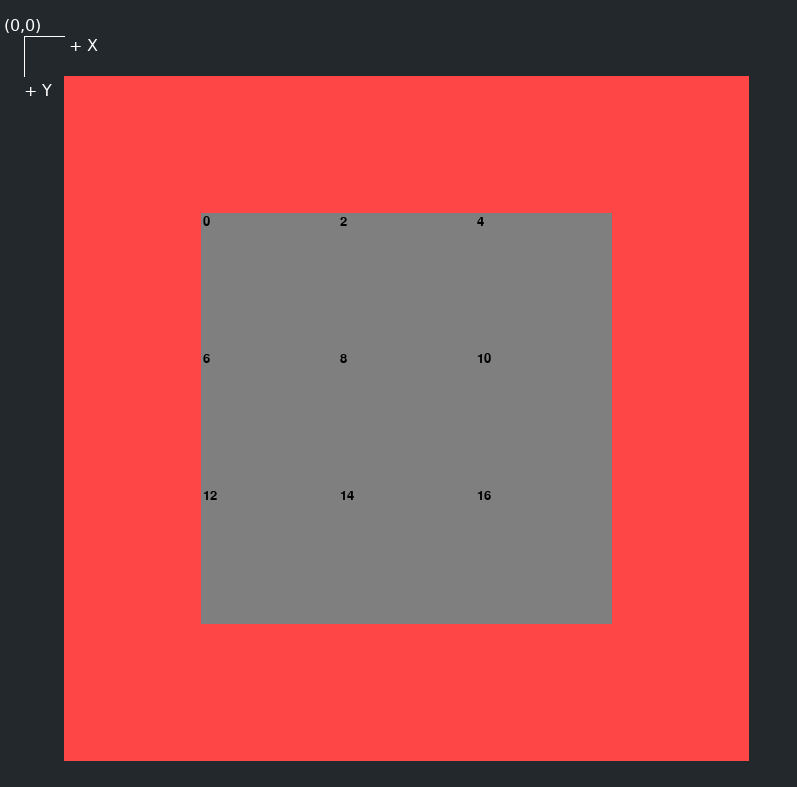
\includegraphics[trim={1.35cm 0 0.9cm 1.5cm}, clip, width=0.6\linewidth]{images/mapa_py.png}
   \caption{Representación de un mapa en Python}
   \label{fig:mapa_py}
\end{figure}

La capacidad de las regiones, es decir, el número de robots que pueden estar simultáneamente en un lugar, se modela mediante los lugares de recursos, a los cuales se les asigna una marca (recurso), cuando el robot entra en una región específica y que se libera cuando el robot deja esa región.

Como ya se ha comentado la aplicación inmediata de los algoritmos implementados para este trabajo es la creación de una plataforma para el control de un sistema multi-robot con el objetivo de evitar colisiones entre los robots móviles. Sin embargo, se puede aplicar a cualquier sistema que sea modelable mediante redes de Petri. Por ello este proyecto tiene trascendencia en todas las áreas del control mediante sistemas de eventos discretos.

Antes de la implementación de uno de estos procesos, es muy importante modelarlo con un sistema discreto, comprobar su funcionamiento y corregirlo si hace falta. Las redes de Petri son una herramienta ampliamente utilizada cuando se trata de sistemas concurrentes, y como en cualquier otro sistema con recursos compartidos pueden aparecer bloqueos, así que este proyecto puede servir para resolver estos bloqueos haciendo el correcto uso de los recursos compartidos y gestionando de forma adecuada su utilización.

Un paso a realizar para obtener el modelo discreto del sistema multi-robot es dividir el mapa en regiones, ya que cada región del mapa se modelará como un lugar en el modelo de la red de Petri o como un nodo en el modelo de un autómata finito determinista. Para resolver el problema mencionado de dividir el mapa en regiones, se utiliza el método de la \textit{Descomposición en celdas}. Este método consiste en dividir las zonas sin obstáculos del plano mediante un cuadrado. Esto se puede ver claramente en la imagen anterior donde las celdas en color gris son las regiones disponibles o habitables por el robot mientras que las celdas rojas representan los límites del mapa.

Una vez descompuesto el mapa en regiones, queda calcular las trayectorias de cada robot para saber porque regiones ha de pasar para alcanzar de la forma más óptima el objetivo prefijado. Las trayectorias son obtenidas de forma automática a partir de algoritmos de cálculo de trayectorias individualmente para cada uno de los robots ignorando al resto de ellos utilizando algoritmos de búsqueda de caminos mínimos en grafos, o también pueden calcularse mediante algoritmos de planificación multi-robot ignorando las posibles colisiones entre los mismos utilizando programación matemática y modelos de tipo redes de Petri. En nuestro caso optamos por utilizar el algoritmo de $A*$, el cual busca el camino más corto para el robot hacía su destino último.

Si los dos robots individualmente siguen sus propias trayectorias, estos pueden colisionar (plazas ocupadas) ya que sus trayectorias pasan por esas regiones que tienen capacidad unitaria (un solo robot puede haber dentro de ellas en cualquier momento). Para evitar las posibles colisiones, se introducen modos de espera, es decir, se impone que por estas regiones no pueda pasar más de un robot al mismo tiempo, de modo que el segundo en llegar a esas regiones deberá esperar a que el primero salga de esa área.

Para sostener este concepto de regiones con capacidad limitada a las redes de Petri, se introducen lugares adicionales, a los que se les llama lugares de capacidades o de recursos compartidos. Estos lugares contienen inicialmente tantas marcas como capacidad tenga la región, en este caso se asignaran recursos con una marca a los lugares que corresponden a regiones con capacidad unitaria. Esta marca se utiliza para disparar la transición de entrada al lugar con capacidad limitada, y cuando el robot abandona esa zona, la transición de salida de ese lugar libera la marca para que vuelva a ser utilizada por el otro robot. Utilizando este concepto para todos los lugares con capacidad finita, la red quedaría como la siguiente.

\begin{figure}[H]
   \centering
   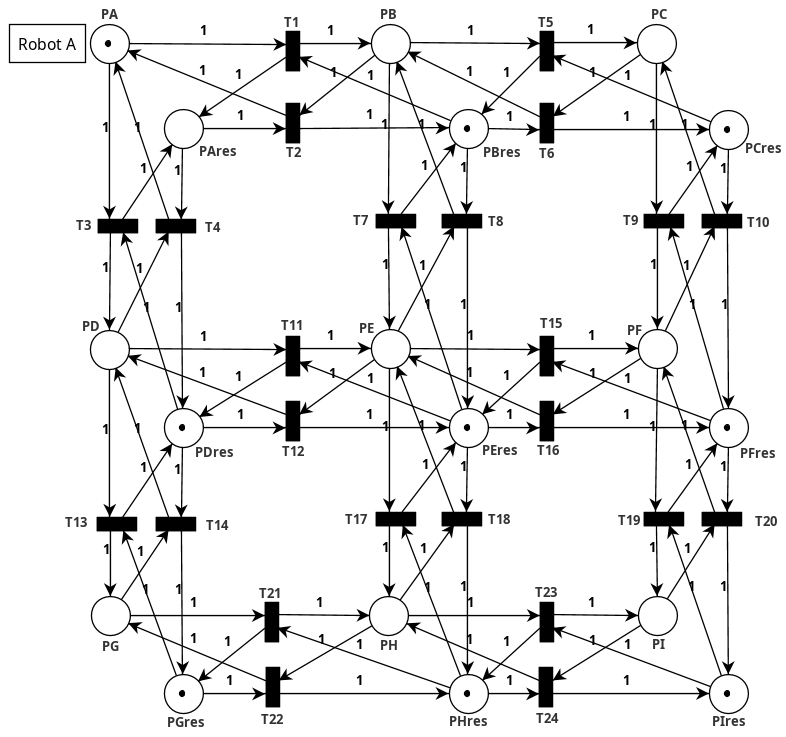
\includegraphics[width=0.8\linewidth]{images/rdp_no_grid.png}
   \caption{Representación del mapa en Python en una red de Petri}
   \label{fig:rdp_no_grid}
\end{figure}

Cabe destacar, que conforme va evolucionando el sistema y los robots se van moviendo de una región a otra, el marcado de la red va cambiando hasta que finalmente cuando un robot termina su trayectoria, la marca vuelve al lugar de reposo, sin embargo, el modelo de  red de Petri no podría volver a ser usado para supervisar el movimiento hasta que el robot sea colocado de nuevo en la posición de inicio del modelo.

Esta simple idea lo que hace es generar modos de espera de modo que nunca puedan coincidir en una región con capacidad restringida más de un robot. De modo que escogiendo correctamente estas regiones en las zonas donde las trayectorias de los robots coinciden, se pueden evitar las colisiones entre robots. Esto es debido a que los recursos compartidos producen modos de espera.

\paragraph{Transformación de un mapa a una red de Petri} \mbox{} \vspace{8pt}

Dentro del programa en Python existe una clase que se encarga de realizar esta transformación, el proceso consiste en definir la estructura que va a tener el mapa, es decir, cuáles van a ser sus espacios habitables y cuáles los límites. Entendiendo cómo límites a las paredes por fuera de la superficie de desplazamiento (su perímetro), y a los obstáculos que pueden existir dentro del mapa (paredes interiores, columnas, objetos, etc). Esto se hace en un archivo de texto que va a ser leído e interpretado por el algoritmo para luego ser convertido en una red de Petri.

\begin{figure}[H]
   \centering
   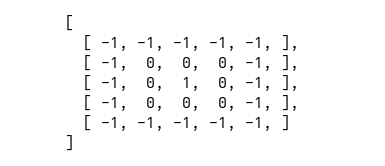
\includegraphics[width=0.5\linewidth]{images/map_definition_matriz.png}
   \caption{Matriz que define el mapa y sus elementos para el programa en Python}
   \label{fig:map_definition}
\end{figure}

La figura \ref{fig:map_definition} muestra el contenido del archivo de texto definido como una matriz de elementos donde, los números $-1$ representan los límites del mapa, los números $1$ los obstáculos y por último los números $0$ los espacios habitables.

El contenido del archivo que se muestra en la imagen anterior es el interpretado por el algoritmo y transformado. De este archivo se obtienen dos definiciones fundamentales para representar de forma correcta y suficiente a la red de Petri. Por un lado la matriz de incidencia, la cual nos describe la relación que existe entre las plazas y las transiciones de la red, es decir, como va a ser el movimiento de los tokens a medida que se disparen las transiciones, y por el otro lado el marcado inicial de la red, es decir, la distribución de los tokens en la red cuando todavía no se disparó ninguna transición. Cómo nosotros buscamos que la red cumpla ciertas condiciones para su adecuado comportamiento (por ejemplo no ser bloqueante), añadimos un lugar de recurso y un lugar de ocupación para celda habitable del mapa, es por ello que la imagen \ref{fig:rdp_no_grid} luce de esa manera.

Todo el proceso de transformación se encuentra descrito en la siguiente imagen, desde la lectura del archivo donde se define la estructura del mapa, pasando por su conversión a las matrices de incidencia y marcado, y por último en cómo el monitor toma esa red de Petri para decidir sobre el avance de los robots en el mapa.

\begin{figure}[H]
   \centering
   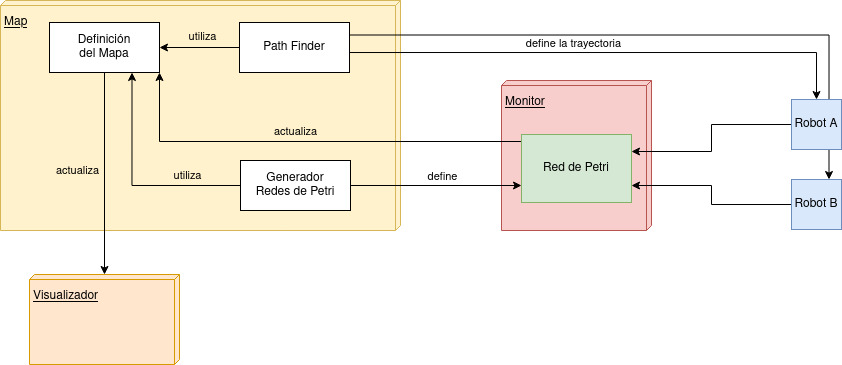
\includegraphics[width=1.0\linewidth]{images/diagrama_clase_monitor.jpg}
   \caption{Diagrama de alto nivel de la transformación de un mapa a una red de Petri}
   \label{fig:mapa_to_rdp}
\end{figure}

\subsubsection{Concurrencia en Python}

Python ofrece diversas formas de manejar la concurrencia, permitiendo que múltiples tareas se ejecuten de manera simultánea. Las principales herramientas para lograrlo incluyen hilos, procesos y asincronía. Sin embargo, la concurrencia en Python está influenciada y controlada por el \textit{Global Interpreter Lock (GIL)}, el cual impide que múltiples hilos ejecuten código Python puro en paralelo dentro de un mismo proceso. Esto influye en su rendimiento ya que todos los hilos, excepto en algunas ocasiones como en las operaciones de entrada/salida, se van a ejecutar en un solo procesador y por lo tanto no se aprovecha todo el potencial de un computador. \cite{lanaro2017python}

El módulo threading permite la ejecución concurrente de tareas dentro del mismo proceso, pero debido al GIL, los hilos no pueden aprovechar múltiples núcleos para realizar cómputo intensivo. Aun así, el threading sigue siendo útil, y sobre todo en el enfoque que estamos tomando para su utilización. Aclarando, los hilos pueden aprovechar el tiempo en el que un proceso está inactivo esperando información, permitiendo la ejecución de otras tareas en paralelo.

Por otro lado, cuando se requiere ejecutar tareas que demandan un alto uso de CPU, la mejor alternativa es el multi procesamiento, que crea procesos independientes con su propio intérprete de Python, evitando la restricción del \textit{GIL} y permitiendo una ejecución realmente paralela.

Teniendo en cuenta que este proyecto está pensado para que escale en cantidad de robots, y se pueda controlar una flota de ellos, se ha optado por utilizar threading debido a que cada hilo va a representar un robot, cuya gestión va a estar coordinada a través del monitor basado en una Red de Petri. Dado que los robots no requieren cómputo intensivo, sino que dependen principalmente de operaciones de I/O y sincronización de eventos, threading resulta adecuado a pesar de las limitaciones del GIL.

Para garantizar un control ordenado de los hilos, se ha implementado un mecanismo de sincronización mediante Lock, permitiendo bloquear el hilo de un robot cuando este no puede avanzar y continuar con los demás. Este enfoque asegura una ejecución eficiente dentro del marco definido por la red de Petri, optimizando el flujo de trabajo sin afectar la estabilidad del sistema.

\subsubsection{Monitor} \mbox{} \vspace{1pt}

La manera en que controlamos la ocupación de los espacios en el mapa, es decir, cómo evoluciona la trayectoria de cada robot es mediante el disparo de un Monitor implementado en Python. Este es el va a controlar, guiar y realizar la toma de decisiones para que cada robot pueda seguir su trayectoria sin interrumpir a los demás y por lo tanto no bloquear todo el sistema.

Para poder guiar a cada robot en su trayectoria, cada uno va a estar representado por un hilo lógico en el programa en Python. Más precisamente cuando existe un robot en el mundo real y se realiza el proceso de sincronización con el software, este va a crear un objeto (representación de un ente en la Programación Orientada a Objetos) el cual va a contener un conjunto de métodos implementados y entre ellos, la creación de un hilo en Python.

A su vez definimos cuál va a ser el punto de inicio y el punto final, es decir el comienzo del recorrido y el final del mismo, y el mapa es un modelo discreto representado por una Red de Petri. Podemos determinar cuales van a ser la plazas que el robot va a ocupar en un preciso momento y las transiciones que se van a disparar para que este pueda llegar a su destino. Con todos estos elementos le damos al monitor las herramientas para realizar su trabajo y efectuar los métodos que le permitan modificar el marcado de la Red de Petri.

\paragraph{Cola de cortesía} \mbox{} \vspace{5pt}

La manera en que el Monitor ejerce el control de la exclusión mutua dentro de la Red de Petri es mediante el uso de colas, entonces, cuando un hilo (robot) está dentro del monitor y aparece otro hilo que intenta ejecutar otro o el mismo procedimiento, el acceso al Monitor se bloquea e inserta el segundo hilo en una cola de cortesía usando una política FIFO. Cuando el primer hilo abandona el monitor, el segundo hilo (que se encuentra en el primer lugar de la cola) es el seleccionado por el Monitor para ejecutar sus tareas. Si la cola está vacía entonces el Monitor se encuentra libre y cualquier hilo que intente tomar el control de éste último podrá hacerlo sin intervención alguna.

\paragraph{Políticas} \mbox{} \vspace{5pt}

Así como mencionamos más arriba que hacemos uso de las colas del monitor para controlar la exclusión mutua, existe la posibilidad de que dos hilos (robots) intenten acceder a la misma plaza ya que su secuencia de disparos así lo determina. En ese caso vamos a tener que tomar una decisión de qué hilo es que va a lograr apoderarse de la plaza en primer lugar. Para esto hacemos uso de una Política definida por nosotros mismos, a partir de ella un hilo va a tener preferencia sobre otro.

Poniendo el caso en concreto de los robots que comparten un mapa, nos parece más acertada la idea de que un robot pueda terminar su recorrido de forma rápida y efectiva. Es por ello que cada robot va guardando el camino que va atravesando, es decir, las celdas por las cuales se desplazó y aumentando un contador interno. Este es el parámetro que se usa para determinar qué robot va a tener preferencia sobre otro, entonces, al momento de ocurrir un conflicto entre dos robots que intentan ocupar la misma celda, el Monitor va a evaluar que robot es el que tiene un mayor camino recorrido y elegirlo para ocupar el lugar en disputa.

\paragraph{Solución de conflictos entre robots} \mbox{} \vspace{5pt}

Acá representamos el posible conflicto que puede ocurrir cuando dos robots intentan ocupar el mismo lugar, como se representan en el mapa y su traducción en una Red de Petri.

\begin{figure}[H]
    \centering
    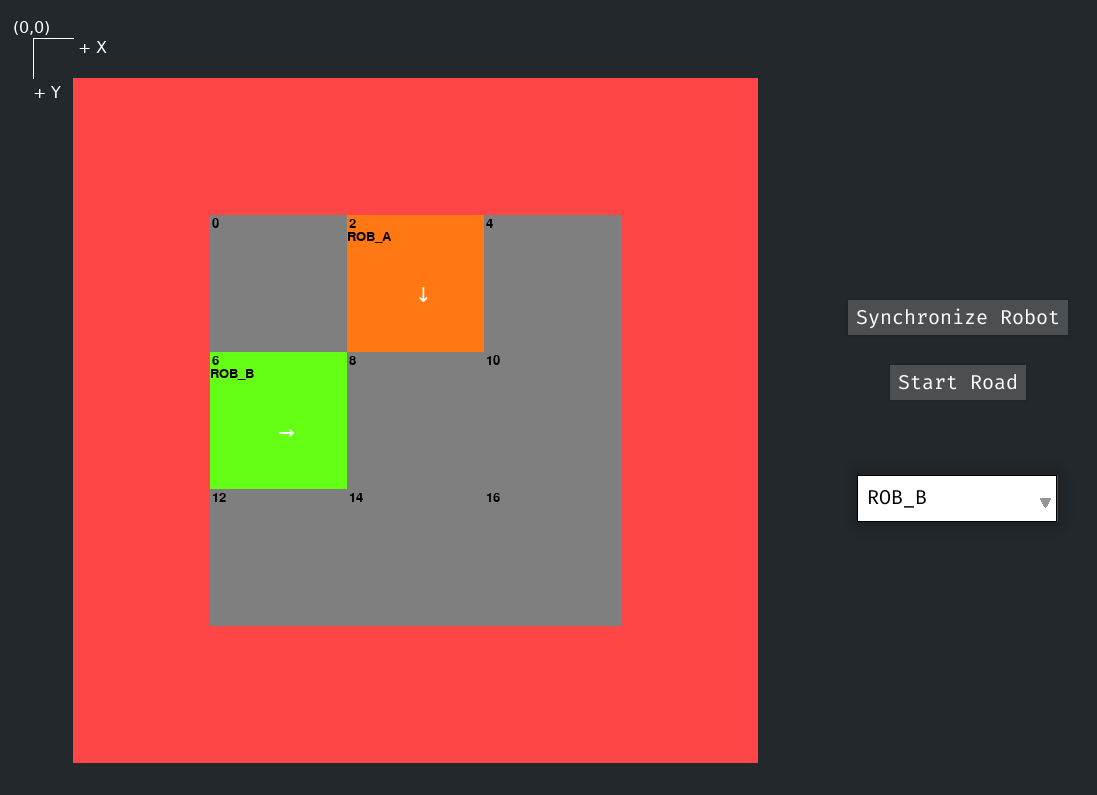
\includegraphics[width=0.7\linewidth]{images/conflicto_map.png}
    \caption{Representación de un conflicto entre dos robots que intentan pasar por la misma celda}
    \label{fig:conflicto_map}
\end{figure}

\begin{figure}[H]
    \centering
    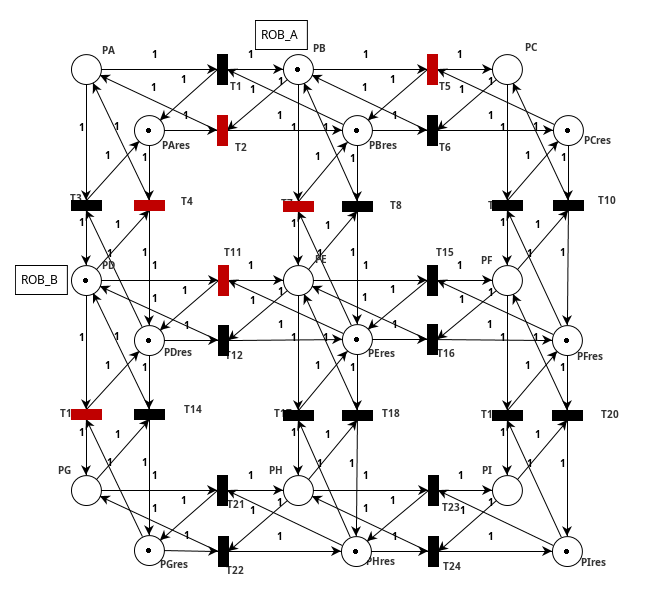
\includegraphics[width=0.7\linewidth]{images/rdp_no_grid_conflicto.png}
    \caption{Representación del conflicto de la figura \ref{fig:conflicto_map} en una red de Petri}
    \label{fig:rdp_no_grid_conflicto}
\end{figure}

\begin{figure}[H]
    \centering
    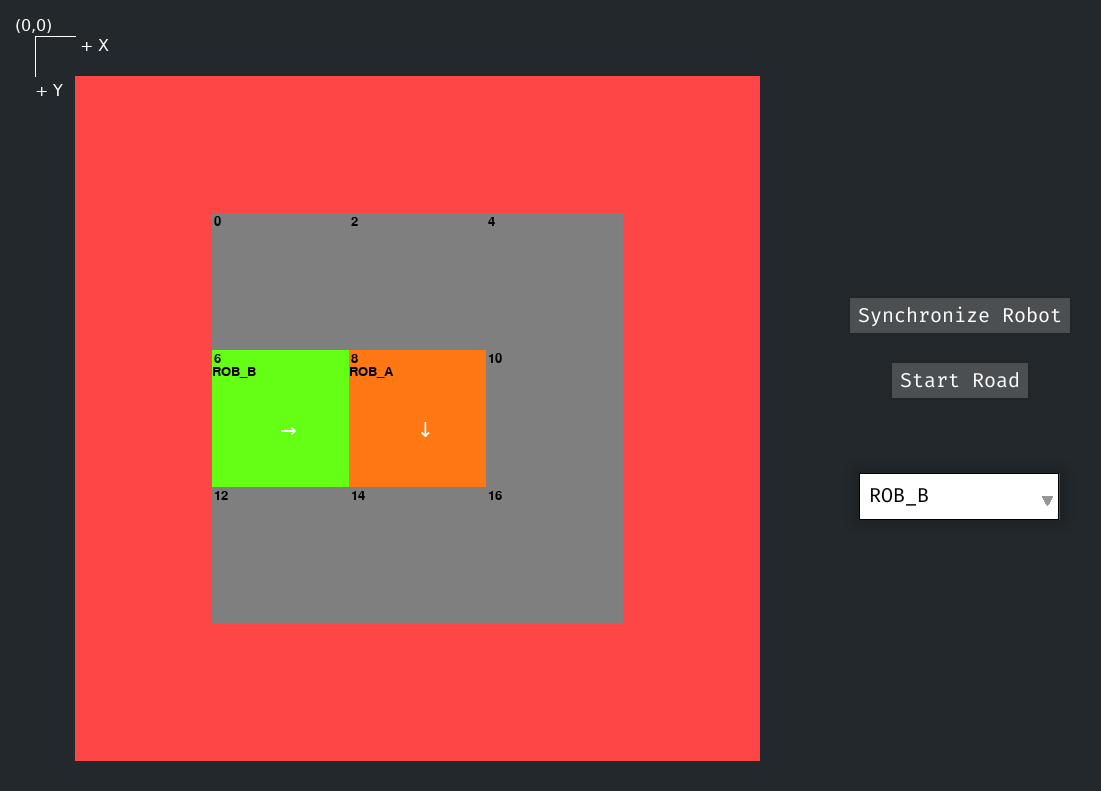
\includegraphics[width=0.7\linewidth]{images/conflicto_map_solucionado.png}
    \caption{Resolución del conflicto de dos robots intentando pasar por la misma celda}
    \label{fig:conflicto_map_solucionado}
\end{figure}

\begin{figure}[H]
    \centering
    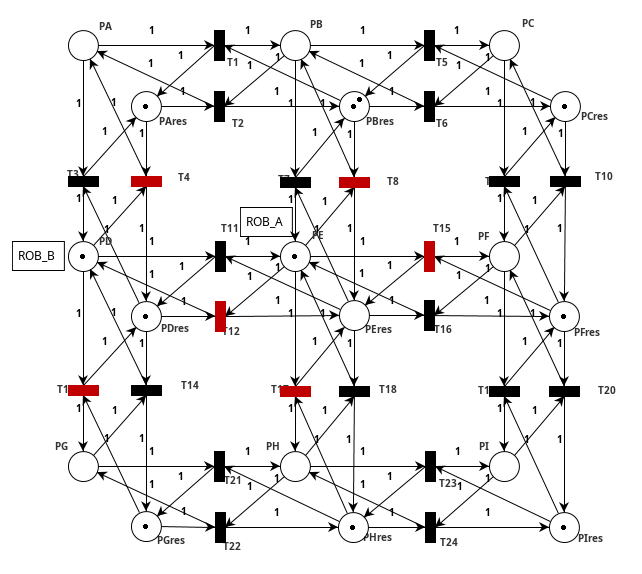
\includegraphics[width=0.7\linewidth]{images/rdp_no_grid_conflicto_solucionado.png}
    \caption{Resolución del conflicto entre los robots representado en una red de Petri y con el nuevo marcado de la red}
    \label{fig:rdp_no_grid_conflicto_solucionado}
\end{figure}

\paragraph{Funcionamiento del monitor} \mbox{} \vspace{10pt}

El funcionamiento del módulo del Monitor en Python queda representado en el siguiente Diagrama de secuencia.

\begin{figure}[H]
    \centering
    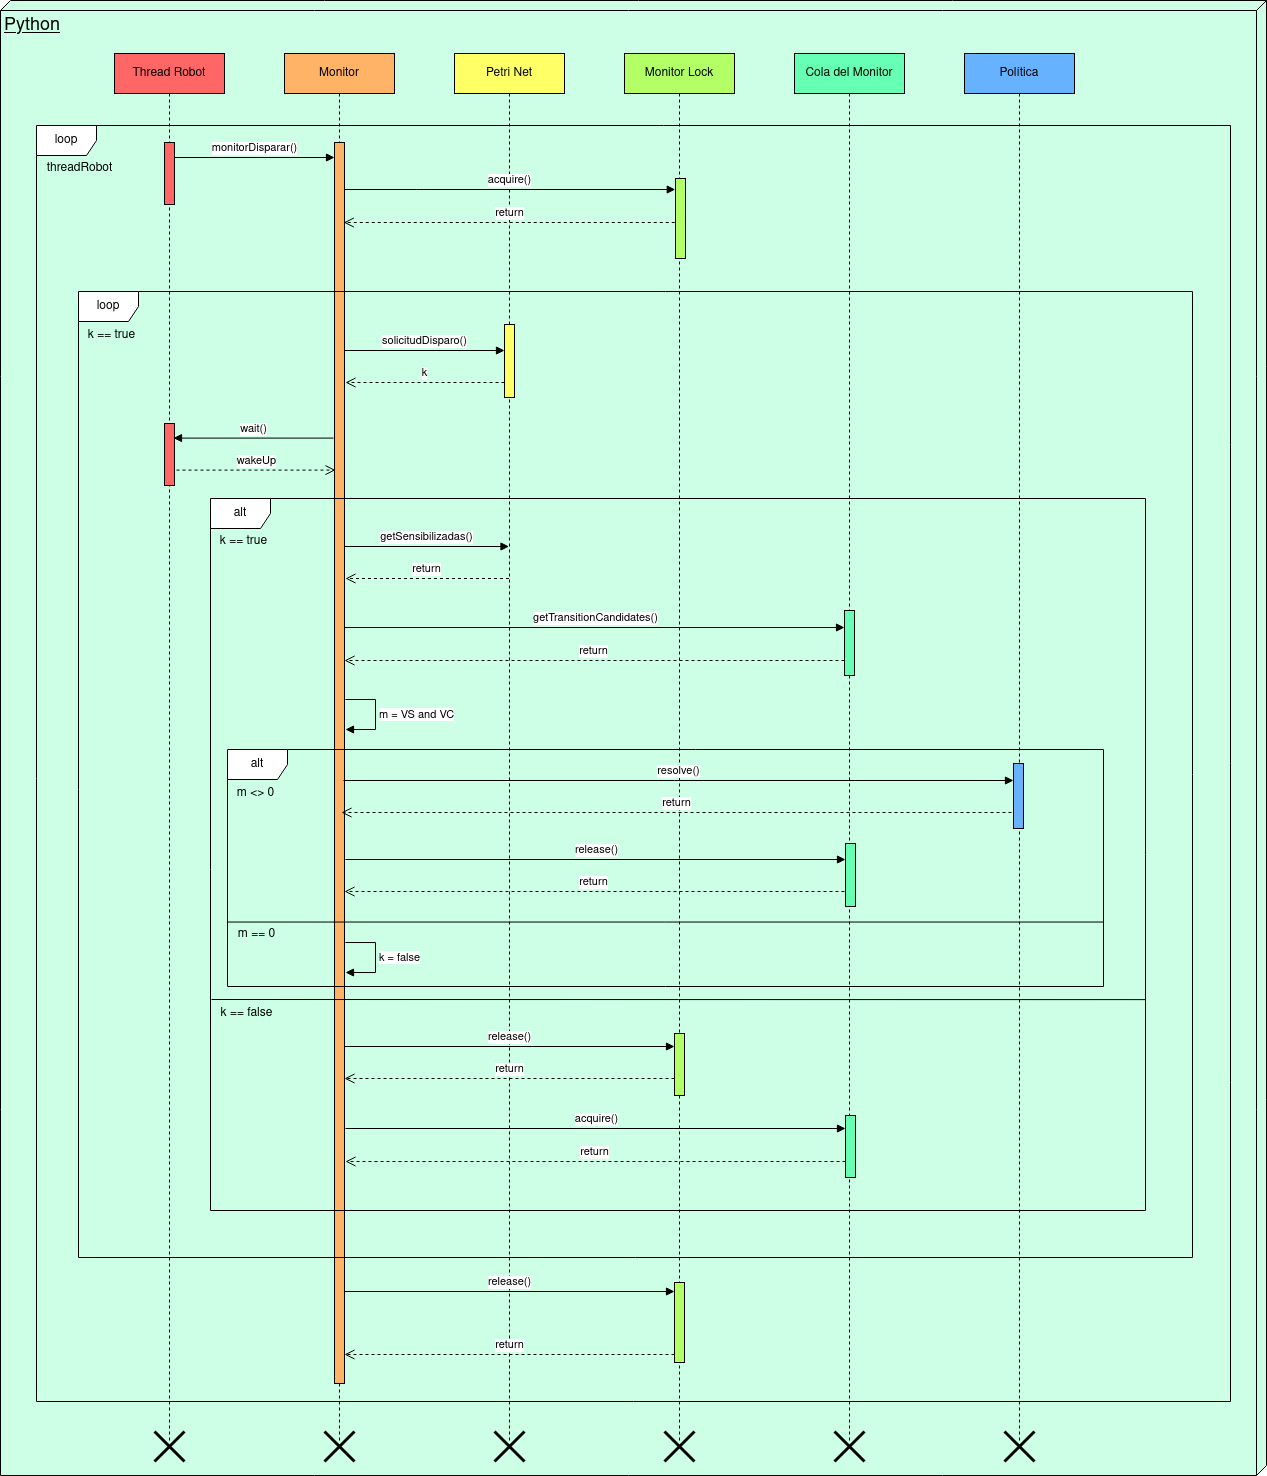
\includegraphics[width=1.0\linewidth]{images/diagrama_monitor.drawio.png}
    \caption{Diagrama de secuencia del monitor}
    \label{fig:diagrama_monitor}
\end{figure}

\subsection{Testing y pruebas}

Las pruebas que se realizaron para que efectivamente podamos determinar el correcto funcionamiento del Monitor, la gestión de la cola de cortesía y la resolución de conflictos mediante la aplicación de una Política fue con la ayuda de la Red de Petri sumamente conocida como Productor-Consumidor. Esta se tomó cómo referencia ya que permite evaluar los problemas de sincronización, concurrencia y gestión de los recursos, entonces, nos pareció un buen puntapié para validar el funcionamiento con un modelo conocido y sumamente usado. Cabe destacar que realizamos la simulación sobre esta red alrededor de $1M$ de disparos y por supuesto siempre validando el resultado de los $P\ invariantes$ y $T\ invariantes$.

\begin{figure}[H]
   \centering
   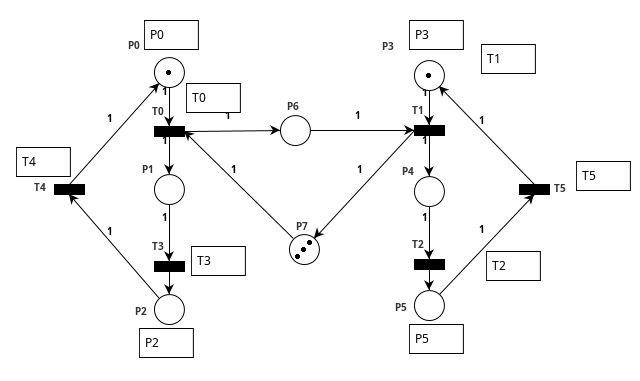
\includegraphics[width=0.9\linewidth]{images/rdp_prod_cons.png}
   \caption{Red de Petri productor-consumidor}
   \label{fig:rdp_prod_cons}
\end{figure}

Se plantearon los siguientes casos:

\begin{testtableformat}
   \hline \rowcolor{test_header_color}
       Test ID             & TC\_04\_00 \\
   \hline
       Tipo de test        & Test unitario \\
   \hline
       Objeto de prueba    & Disparar las transiciones sensibilizadas del Productor \\
   \hline
       Nombre              & Ejecución del productor \\
   \hline
       Descripción         & Realizar el disparo de las transiciones sensibilizadas del productor teniendo como máximo 3 (tres) tokens disponibles para producir\\
   \hline
       Precondición        & PRECOND\_D \\
   \hline
       Pasos del test      & \begin{enumerate}
                             \item Instanciar a la clase monitor con la red productor-consumidor
                             \item Obtener el vector de transiciones sensibilizadas 
                             \item Ejecutar un disparo de la transición sensibilizada 
                             \item Adquirir el marcado saliente y compararlo con un programa de análisis de redes de Petri 
                             \end{enumerate}\\
   \hline
       Resultado esperado  & El marcado en ambos casos debe coincidir \\
   \hline
       Resultado obtenido  & El marcado de la red obtenido por la clase monitor y el programa de análisis de redes de Petri son iguales, por lo tanto, se verifica su adecuado funcionamiento \\
   \hline
       Observaciones       & -\\
   \hline
\end{testtableformat}

\begin{testtableformat}
   \hline \rowcolor{test_header_color}
       Test ID             & TC\_04\_01 \\
   \hline
       Tipo de test        & Test unitario \\
   \hline
       Objeto de prueba    & Disparar las transiciones sensibilizadas del consumidor \\
   \hline
       Nombre              & Ejecución del consumidor \\
   \hline
       Descripción         & Realizar el disparo de las transiciones sensibilizadas del consumidor teniendo como máximo 3 (tres) recursos disponibles generados por el productor\\
   \hline
       Precondición        & PRECOND\_D \\
   \hline
       Pasos del test      & \begin{enumerate} 
                             \item Instanciar a la clase monitor con la red productor-consumidor 
                             \item Obtener el vector de transiciones sensibilizadas 
                             \item Ejecutar un disparo de la transición sensibilizada 
                             \item Adquirir el marcado saliente y compararlo con un programa de analisis de redes de petri 
                             \end{enumerate}\\
   \hline
       Resultado esperado  & El marcado en ambos casos debe coincidir \\
   \hline
       Resultado obtenido  & El marcado de la red obtenido por la clase monitor y el programa de análisis de redes de Petri son iguales, por lo tanto, se verifica su adecuado funcionamiento \\
   \hline
       Observaciones       & -\\
   \hline
\end{testtableformat}

\begin{testtableformat}
   \hline \rowcolor{test_header_color}
       Test ID             & TC\_04\_02 \\
   \hline
       Tipo de test        & Test unitario \\
   \hline
       Objeto de prueba    & Disparar una transición con política de decisión \\
   \hline
       Nombre              & Ejecución de una transición con política definida \\
   \hline
       Descripción         & En en el caso donde tanto el productor cómo el consumidor pueden disparar una transición, la idea es evaluar la política de la transición del consumidor para que tenga prevalencia sobre el productor ante una situación indeterminista \\
   \hline
       Precondición        & PRECOND\_E \\
   \hline
       Pasos del test      & \begin{enumerate} 
                             \item Instanciar a la clase monitor con la red productor-consumidor 
                             \item Generar una situación de equidad donde ambos recursos puedan disparar su transición 
                             \item Obtener el vector de transiciones sensibilizadas 
                             \item Evaluar la política de las transiciones sensibilizada y elegir cual disparar 
                             \item Ejecutar un disparo de la transición elegida 
                             \item Adquirir el marcado saliente y compararlo con un programa de análisis de redes de petri 
                             \end{enumerate}\\
   \hline
       Resultado esperado  & El marcado actual en ambos casos debe coincidir y la transición disparada debe ser la del consumidor \\
   \hline
       Resultado obtenido  & El marcado de la red obtenido por la clase monitor y el programa de análisis de redes de Petri son iguales, por lo tanto, se verifica su adecuado funcionamiento \\
   \hline
       Observaciones       & -\\
   \hline
\end{testtableformat}

\begin{testtableformat}
   \hline \rowcolor{test_header_color}
       Test ID             & TC\_04\_03 \\
   \hline
       Tipo de test        & Test integración \\
   \hline
       Objeto de prueba    & Realizar movimientos con el robot dentro del mapa, el robot sólo va a avanzar cuando la red de Petri haya hecho la solicitud de disparo y haya verificado que el robot no se encuentra bloqueado.\\
   \hline
       Nombre              & Desplazamientos del robot controlado por el Monitor\\
   \hline
       Descripción         & Para que el robot avance de una celda a otra y realice el desplazamiento definido (punto inicial y final) debe ser autorizado y coordinado por el monitor que controla la red de Petri.\\
   \hline
       Precondición        & PRECOND\_E \\
   \hline
       Pasos del test      & \begin{enumerate}
                             \item Indicar los puntos de inicio y final del robot
                             \item Esperar que el Monitor dispare la transición sensibilizada
                             \item El robot recibe la orden de avanzar a la celda libera
                             \item El robot envía una señal de llegada a la celda (plaza)
                             \item Se dispara la siguiente transición sensibilizada
                             \item Este proceso se repite hasta que el robot llegue a su destino
                             \end{enumerate}\\
   \hline
       Resultado esperado  & El robot pueda completar su desplazamiento definido por el usuario\\
   \hline
       Resultado obtenido  & La red de Petri al no bloquearse permite que todas las transiciones sensibilizadas se puedan disparar y por ende que el robot pueda desplazarse por todas las celdas (plazas) involucradas en su recorrido\\
   \hline
       Observaciones       & -\\
   \hline
\end{testtableformat}

\begin{testtableformat}
    \hline \rowcolor{test_header_color}
        Test ID             & TC\_04\_04 \\
    \hline
        Tipo de test        & Test de sistema \\
    \hline
        Objeto de prueba    & Comunicación inalámbrica - PID - Modelo cinemático - Odometría - Seguidor de línea magnética - Modelo del mapa - Calculador de trayectorias - Interfaz de usuario - Red de Petri - Monitor \\
    \hline
        Requerimiento       & RF1 - RF2 - RF3 - RF4 - RF5 - RF6 - RF7 - RF10 \\
    \hline
        Nombre              & Prueba de sistema integrado\\
    \hline
        Descripción         & Comprobar que el robot se puede desplazar por el mapa gestionado por el marcado de la red de Petri\\
    \hline
        Precondición        & PRECOND\_G \\
    \hline
        Pasos del test      & \begin{enumerate}
                              \item Indicar los puntos de inicio y final del robot en el mapa
                              \item Calcular la secuencia de disparos del Monitor
                              \item Esperar que el Monitor dispare la transición sensibilizada
                              \item El robot recibe la orden de avanzar a la celda (plaza) liberada
                              \item El robot envía una señal de llegada a la celda (plaza) destino
                              \item Se dispara la siguiente transición sensibilizada
                              \item Este proceso se repite hasta que el robot llegue a su destino
                              \end{enumerate}\\
    \hline
        Resultado esperado  & El robot pueda completar su desplazamiento definido por el usuario\\
    \hline
        Resultado obtenido  & La red de Petri al no bloquearse permite que todas las transiciones sensibilizadas se puedan disparar y por ende que el robot pueda desplazarse por todas las celdas (plazas) involucradas en su recorrido\\
    \hline
        Observaciones       & Se probó recorridos de 4 de metros por limitaciones de espacio\\
    \hline
 \end{testtableformat}

\subsection{Resultados}
Como muestran las pruebas realizadas del módulo Monitor implementado en Python, el algoritmo se comporta de forma correcta y las validaciones realizadas sobre la red de Petri, productor-consumidor, entregaron los resultados suficientes para poder llevar este procedimiento a las redes que representan los mapas donde los robots se van a desplazar y tener la validez que el monitor va a permitir que estos se muevan de forma coordinada y puedan llegar a su destino.

\subsection{Riesgos superados}

\begin{center}
    \begin{tabular} {
        | c| c |}
        \hline \rowcolor{test_header_color}
            ID & Riesgo \\
        \hline
            RI-02 & Intercomunicación de componentes ineficiente o ineficaz \\
        \hline
            RI-03 & Prestaciones insuficientes de componentes \\
        \hline
    \end{tabular}
\end{center}

\subsection{Conclusiones}
El desarrollo del sistema de control para robots omnidireccionales, basado en redes de Petri, demostró ser altamente efectivo en la gestión de trayectorias y prevención de colisiones en entornos multi-robot. Mediante la discretización del mapa en celdas y su representación como lugares en la red, se logró un modelo claro y funcional que garantiza la ocupación exclusiva de regiones con capacidad limitada. La implementación de políticas de prioridad dinámica, donde los robots con mayor recorrido tienen preferencia, permitió resolver conflictos de manera eficiente, evitando bloqueos y asegurando un flujo continuo de operaciones.

En síntesis, el sistema desarrollado no solo cumple con los requerimientos funcionales y no funcionales planteados, sino que también sienta las bases para extensiones más complejas, destacando la versatilidad de las redes de Petri en el ámbito del control y la automatización.